\chapter{Introduction and Quickstart}\label{cha:introduction}
This document is a pilot's manual for XCSoar, an open-source glide
computer originally developed for Pocket PC devices.  The audience 
is assumed to have a sound knowledge of the fundamental theory of flight for
gliders, and at least a basic working knowledge of cross-country soaring.

Updates to the XCSoar software may result in some of this manual being
out of date. You should read the release notes distributed with the
software to keep track of changes.  Updates to the manual and software
are available from 
\begin{quote}
\xcsoarwebsite
\end{quote}

\section{Organization of this manual}

\todonum[inline]{Write about the manual crossref hinting icons and the yellow
colour. The Quickstart will be readable also without those links available} 
This manual is broadly
organized into the major functions of the software from a pilot's perspective.  The remainder of this chapter
deals with how to download, install and run the software on various
platforms.  Chapter~\ref{cha:interface} introduces the user interface
concepts and gives an overview of the display.

Chapter~\ref{cha:navigation} describes the moving map part of the
display in greater detail and describes how the software can assist in
general navigation.  Chapter~\ref{cha:tasks} describes how
cross-country tasks are specified and flown, and presents some of the
analysis tools available to pilots to help improve their performance.
Chapter~\ref{cha:glide} goes into further detail on the glide computer
functions as it is important for pilots to be aware of how the
computer performs its calculations.

Chapter~\ref{cha:atmosph} describes how the computer can interface to
variometers and other air data sensors, and how it uses these
measurements to provide various models of the atmosphere, in
particular on winds and thermal convection.
Chapter~\ref{cha:airspace} describes how XCSoar can assist in managing
flight in special use airspace and the FLARM collision awareness
system.  Chapter~\ref{cha:avionics-airframe} deals with systems
integration and systems diagnostics, the integration of XCSoar with
communications devices and with airframe switches.

The remainder of the manual contains mainly reference material.
Chapter~\ref{cha:infobox} lists the types of information that can be
displayed in the grid of InfoBoxes next to the map display.  The
configuration of the software is described in detail in
Chapter~\ref{cha:configuration}.  The formats of the various data
files that program uses, as well as where to obtain them from and how
to edit them, is described in Chapter~\ref{cha:data-files}.

Finally, a short history and discussion of XCSoar's development
process is presented in Chapter~\ref{cha:history-development}.

\section{Notes}

\subsection*{Terminology}
A variety of terms may be used to describe embedded devices like the Pocket PC
platform, including `organiser', Portable Digital Assistant (PDA)
and Personal Navigation Assistant (PNA).  XCSoar is
also available on Triadis Engineering's Altair glide computer, which is
formally an Electronic Flight Instrumentation System, and several other
platforms. Throughout this document, these terms are used interchangeably to
refer to whatever hardware XCSoar is running on.

\subsection*{Screenshots}
Throughout this manual are several screenshots of XCSoar. These are
taken from the program running on a variety of hardware platforms and possibly
even different versions. Each platform and version may have different screen
resolutions, layouts and fonts, and so there may be slight differences in the
appearance of the display. Most of the screenshots in this manual are taken of
XCSoar running in landscape orientation.

\section{Platforms}
\begin{description}
\item[Windows PC]
It is possible to run XCSoar on an ordinary computer with the Windows
operating system. This setup can be used for training yourself in using XCSoar.
A simulation mode is included in XCSoar as well as a IGC replay function, that
can be used when not connected to a valid GPS source.
\item[Windows Mobile PDA/PNA]
Devices powered by Microsoft Pocket PC 2000 up to Windows Mobile 6 are
supported by XCSoar. Windows Mobile 7 will not be supported as Microsoft decided
to skip support for native applications from this version on.
\item[Unix/Linux PC]
XCSoar can be run on Unix using the Wine emulator. A native Unix port
has been released with the 6.0 version of XCSoar, but is still
considered experimental.
\item[Android Devices]
XCSoar runs on Android 1.6 or newer.
\item[Altair]
The Altair glide computer by Triadis Engineering is a glide computer
factory installed with XCSoar.  The Altair PRO version also contains
an internal GPS.
\end{description}

\section{Downloading XCSoar}
The software is available as a free download from the XCSoar website
~\xcsoarwebsite. Follow the links to the download section.

\subsection*{Pocket PC versions}
Download the relevant package for your Pocket PC operating system
version and save it to disk:
\begin{description}
\item[Pocket PC 2000] For Pocket PC 2002 and older
\item[Windows Mobile 2003] For Windows Mobile 2003 (or Pocket PC 2003)
\item[Windows Mobile 5] For Windows Mobile 5 and 6
\end{description}

\subsection*{Data files location}
To be able to use XCSoar's advanced features, additional data files, such as
terrain, topography, special use airspace, waypoints etc.\ are needed. The files
that can be used with XCSoar are described in Chapter~\ref{cha:data-files}.

All data files should be copied into the directory
\texttt{XCSoarData}.  This directory must be in a specific place
so that XCSoar knows where to look for data files:

\begin{description}
\item[Windows PC]
\texttt{XCSoarData} must be located in your personal folder (``\texttt{My
Documents}'')
\item[Windows Mobile PDA/PNA]
\begin{itemize}
\item If you start XCSoar from a SD card, it is always in the root of
  that SD card (e.g. ``\texttt{SD Card/XCSoarData}'')
\item If \texttt{XCSoarData} already exists on any SD card inserted
  at XCSoar start\-up, this one is used.
\item If none of the above applies, then it is in your personal folder
  (``\texttt{My Documents/}'')
\end{itemize}
\item[Unix PC]
\verb|~/.xcsoar/XCSoarData|.
\item[Android Devices]
\texttt{XCSoarData} is located on the SD card (e.g.
``\texttt{/sdcard/XCSoarData}'').
\item[Altair]
If XCSoarData exists on an USB drive, that one is used, otherwise the
internal storage is used.
\end{description}

For embedded devices it is recommended to create \texttt{XCSoarData} on a SD
card, because you can easily update the data files using your PC.


XCSoar will generate a number of additional files at run time.  These
will be placed in the  \texttt{XCSoarData} directory (Windows PC and 
Windows Mobile devices), or the \texttt{.xcsoar} directory (Unix/Linux
PC).  At first run, XCSoar will create the files 
\texttt{Default.tsk} (Default Task),  \texttt{xcsoar-registry.prf} 
(configuration settings), \newline
\texttt{xcsoar-startup.log} (log of the startup progress), 
plus three directories: \texttt{cache},
\texttt{config} and \texttt{logs}.  Additional files may be
created/modified while XCSoar is running, such as task files
(\texttt{*.tsk}) and flight logs.




\section{Installation}
\subsection*{Installation of Pocket PC version from Windows PC}

Prior to performing any installation, it is a good idea to backup your
organiser for extra safety.

The following sequence describes how to install XCSoar from Windows:
\begin{enumerate}
\item Place your PocketPC in its cradle and make sure
 you have MS ActiveSync running.
\begin{center}
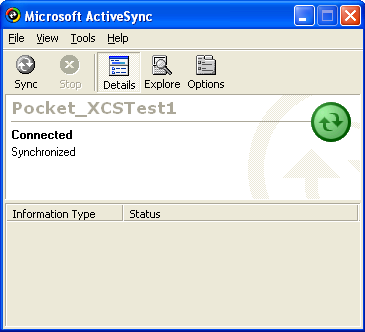
\includegraphics[angle=0,width=\linewidth,keepaspectratio='true']{figures/XCS_ActiveSync.png}
\end{center}

\item Run the program \verb|Install-XCSoar-XXX-YYY.exe| 
  (where XXX and YYY refer to the version number and operating system
  version respectively).

\begin{center}
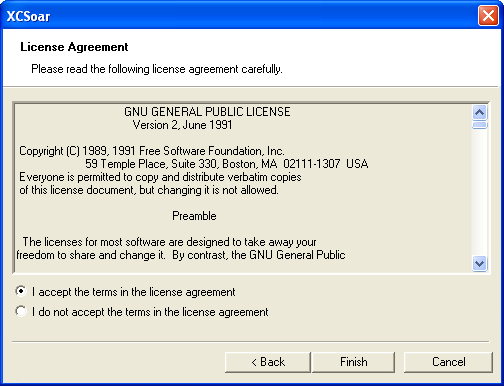
\includegraphics[angle=0,width=\linewidth,keepaspectratio='true']{figures/XCS_License.png}
\end{center}

\item Read and accept the license
\item Follow the prompts in the installation program and also follow the prompts on the organiser.

\begin{center}
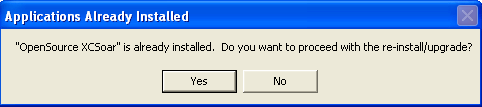
\includegraphics[angle=0,width=\linewidth,keepaspectratio='true']{figures/XCS_Windows.png}
\end{center}

\item XCSoar is now installed.
\item Perform a reset of your device.  See the operating instructions for your
  organiser about how to do this.
\item After the reset, the XCSoar `FLY' and `SIM' launcher icons will
 be visible on the Today screen.

\begin{center}
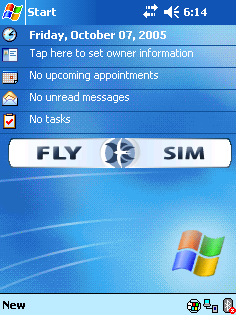
\includegraphics[angle=0,width=0.6\linewidth,keepaspectratio='true']{figures/XCS_Today.png}
\end{center}

\end{enumerate}

It is a good idea to assign one of your PocketPC hardware buttons to
run XCSoar. See your PocketPC manual for details of how to do this.

Owners of Compaq Aero PocketPCs may find it useful to enable `Game
Keys'.

\subsection*{Installation of Pocket PC version from a Pocket PC CAB file}

You can download the CAB file appropriate for your organiser and
install it onto a nonvolatile storage card like a Compact Flash or
Secure Digital card. Place it in your organiser. Use the File Manager
on your organiser to find the CAB and click on it to execute
it. Follow the on-screen instructions, the CAB file will be deleted
after installation.

Alternatively you can download the CAB file from Sourceforge through
your Internet Explorer on your organiser and install it that way.

\tip It is generally a good idea to keep the CAB file on the storage card
so that if the organiser's power fails and the memory is lost, XCSoar
can be reinstalled.

\subsection*{Installation of PC version}

The file \verb|XCSoarPC.zip| needs to be unzipped using a utility
program such as WinZip.

Development of a proper windows installer for the PC version is in
progress.  For now, any additional data files used by the PC version
must be placed in the \verb|My Documents\XCSoarData| directory.


\subsection*{Installation on Unix/Linux}

The file downloaded is \verb|xcsoar_XXX.deb|, where \verb|XXX| includes
the version number and platform, e.g. \verb|xcsoar_6.0.4_i386.deb|.
The is a Debian package and can be installed using 
\begin{center}
\verb|sudo dpkg -i xcsoar_XXX.deb|.
\end{center}
Use \verb|dpkg-query -L xcsoar| to see where the executable and 
other files are installed,
Additional data files must be placed in the directory
\verb|~/.xcsoar/XCSoarData/|.
If \verb|~/.xcsoar| does not exist, it will be created the first time
that \verb|xcsoar| is run.


\subsection*{Installation on Android}

Obtain XCSoar from Google's Android market, or install the \verb|apk|
file manually.  Copy the data files on the SD card in the directory
\verb|XCSoarData|.




\section{Running XCSoar}
%\subsection*{Fly and simulator modes}

Two modes are available inside the XCSoar application: 
\begin{description}
\item[FLY] This mode is used when actually flying.  The simulator is 
  disabled and serial communications are active. 
\item[SIM] This starts XCSoar in simulator mode, no serial communications
  are attempted.
\end{description}

\subsection*{XCSoar Pocket PC version}
The program can be run in either of two modes by pressing the `FLY' or
`SIM' launcher on the Today screen. If the application is started directly from
the explorer a dialog is asking you which mode you want to start.

\tip It is recommended that on Pocket PC devices, no other programs
 are running while XCSoar is used in flights.  This gives the best
 possible performance and responsiveness of the program.

\subsection*{Altair version}
XCSoar starts up automatically when Altair is powered on.
The PWR/ESC button (top left) has multiple functions:
\begin{description}
\item[Powering on]  Press and hold the PWR/ESC button for one second.
  The LED in the button will light up, and XCSoar will start after
  Altair has booted.
\item[Powering off]  Press and hold the PWR/ESC button for 3 seconds.
  Altair will switch off.
\item[Escape] Pressing the PWR/ESC button quickly acts as an
Escape key, typically used to close dialog pages or as a cancel function.
\end{description}

The Altair version of XCSoar does not include a simulator mode.

\subsection*{XCSoar PC version}
The program can be run by opening the explorer window, finding the directory
that has the XCSoar.exe executable, and double clicking on that program file.

The program command line options allows the screen orientation of
the display to be defined:
\begin{description}
\item[-portrait] The screen is 480 pixels wide, 640 pixels high.
\item[-square] The screen is 480 pixels wide, 480 pixels high.
\item[-landscape] The screen is 640 pixels wide, 480 pixels high. This is the
usual setting. If you don't specify this parameter the landscape version will be
loaded automatically.
\item[-small] Draws the screen at half size.  This is useful for using XCSoar in
 conjunction with flight simulators e.g.\ Condor.
\end{description}
To change the screen orientation, it is convenient to create a shortcut to the
program, then right click on the shortcut icon and click on ``Shortcut''. 
In the field ``Target'' add one of the desired options listed above.

\subsection*{XCSoar Unix/Linux PC version}
Run \verb|xcsoar| from a command line, or create a shortcut on the
desktop.  The location of the executable file may be found using
\verb|which xcsoar|.  Only landscape mode is  supported for now.

\subsection*{Loading data files}
The first time that XCSoar is run, it does not automatically load the 
data files that you placed in the \verb|XCSoarData| directory.  
To tell XCSoar which files to load, double click/tap the map (the large,
blank white part with the glider symbol in the center),
choose the menu \bmenu{Config} (click/tap it twice), then select
\bmenu{System Setup}.  The System Setup screen should be displayed:
\begin{center}
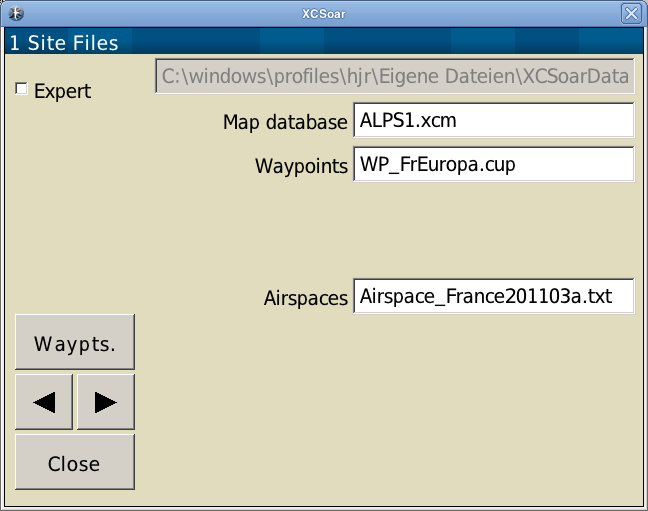
\includegraphics[angle=0,width=0.8\linewidth,keepaspectratio='true']{figures/config-basic.png}
\end{center}
The first page allows you to choose the map, 
waypoint and airspace files, by clicking/tapping on the text boxes.
Many other features of XCSoar may be configured with
\bmenu{System Setup}. These are described in detail in Chapter
\ref{cha:configuration}.
Once completed, XCSoar must be restarted; from now on, the data files
will be loaded automatically at run time.

\subsection*{Start-up and user profiles}
When XCSoar starts up, it will check for existing profiles. If multiple
profiles are detected it will displays a small window asking you which profile
to load. To proceed, choose the desired profile and press Enter. If no
profile is chosen the settings from the last session are loaded again. Profiles
can be useful for example in the following cases:
\begin{itemize}
\item Different pilots
\item Competition versus casual flying
\item Flying in different locations
\end{itemize}


\subsection*{SIM mode}
The simulator contains a simple interface allowing the user to fly
the glider about.  On the map screen, clicking/touching the glider symbol
(with touchscreen or mouse) and dragging 
causes the glider to move in the direction of the drag, the
speed being proportional to the length of the drag.  

In the PC version and for embedded devices with buttons, the aircraft
speed, height and direction may be changed using the \InfoBox es.
These features are not available for touchscreen devices.
The aircraft altitude can be adjusted by selecting the GPS altitude
{\InfoBox} (marked \infobox{H GPS}), and pressing the up or down key.
The airspeed  can be adjusted by selecting the ground speed
{\InfoBox} (marked \infobox{V Gnd}), and pressing the up or down key.
The glider's track  can be adjusted by selecting the track
{\InfoBox} (marked \infobox{Track}), and pressing the up or down key.
With either of the \InfoBox es \infobox{H GPS} or \infobox{V Gnd})
selected, the glider's direction may be changed using the left/right keys.

Other controls, buttons and menus work the same as in FLY mode.


\subsection*{Splash screen}
When XCSoar starts up, shuts down, or loads large files, such as airspace,
waypoints, terrain, etc., a progress screen is presented while the data is being
loaded. This screen has a progress bar which indicates the data loading
activity, and a short line of text describing the action that is being performed.

This screen also displays the software version information.

\subsection*{Exiting the program}
For PDA and PC versions, XCSoar is shut down from the menu. The menu can be
opened by double-clicking on the map or the \InfoBox es.
\begin{quote}
\bmenu{QUIT}
\end{quote}

For PC versions, XCSoar can also be shut down by clicking the close icon
on the XCSoar window.

For Altair, XCSoar is shut down by holding the PWR button for two seconds or
more.





\section{Technical support}

\subsection*{Troubleshooting}
A small team of dedicated developers produces XCSoar. Although we are
happy to help with the use of our software, we cannot teach you about
basics of modern information technology. If you have a question about XCSoar in
particular please email us at: 
\begin{quote}
\url{xcsoar-user@lists.sourceforge.net}.
\end{quote}

Any frequent questions will be added to this document and to the Frequently
Asked Questions (FAQ) section of the XCSoar website.

You may also find it useful to subscribe to the XCSoar users mailing
list so you will be kept up to date with latest developments. You can find more
information about the XCSoar mailing lists on our website:
\begin{quote}
\xcsoarwebsite
\end{quote}

A log file of the startup progress of XCSoar is generated in the file
\verb|xcsoar-startup.log|. This can be sent to the XCSoar developers
to help determine the cause of any startup related problems.

For Altair users, the startup file is transferred to the `FromAltair'
directory by AltairSync if a USB drive is plugged in when Altair is
first switched on.

\subsection*{Updates}
You should periodically visit the XCSoar website to check for program
updates. The installation procedure described above can typically be
repeated in order to upgrade the software.  All user configuration
settings and data files will be preserved during the
re-installation/upgrade.

It is also recommended to periodically check for updates to data
files, particularly Special Use Airspace, which may be subject to
change by the national civil aviation authority.

Like any complex software program, XCSoar may be subject to software
bugs, so if you find any, please report them to the XCSoar developers
by using our bug tracker ``trac'' at 
\begin{quote}
\url{http://www.xcsoar.org/trac/}
\end{quote}
or by sending an email to
\begin{quote}
\url{xcsoar-devel@lists.sourceforge.net}
\end{quote} 

\subsection*{Updating XCSoar on Altair}
Updating XCSoar on Altair involves downloading the latest program file
{\tt XCSoarAltair-YYY-CRCXX.exe}, copying it to a USB memory stick,
then using the AltairSync utility on the Altair device to complete the
installation.  Refer to the {\em Altair Owner's Manual} for details.

Other data and program files can be transferred to Altair in a similar
way.

\section{Training}
For the safety of yourself and others, pilots using XCSoar are advised to
train themselves in using XCSoar on the ground and become familiar with its
interface and features prior to flight.

\subsection*{Using XCSoar on the PC}
The PC versions of XCSoar may be used to become familiar with XCSoar's
interface and functionality in the comfort of one's home.  All files
and configuration used by this version are identical to the embedded versions,
so it can be helpful to try out customisations on the PC version before using
them in flight.

The PC versions can also be connected to external devices and operate just as
the embedded versions do. Suggested uses include:
\begin{itemize}
\item Connect the PC to a FLARM device to use XCSoar as a ground
station display of FLARM-equipped traffic.
\item Connect the PC to an intelligent variometer such as Vega to
test configuration settings of the variometer.
\end{itemize}

\subsection*{Using XCSoar with a flight simulator}
A good way to learn how to use XCSoar is to connect the Pocket PC
device to a PC running a flight simulator that can output NMEA
sentences to the serial port. Suitable simulators include Condor and
X-Plane.  

The benefit of this form of training is that XCSoar can be used in FLY
mode, so it behaves exactly as if you were really flying, and you can
get a good feel for how the program works while you are flying the
simulator.

\section{Using XCSoar safely}
The use of an interactive system like XCSoar in flight carries with it
certain risks due to the potential distraction of the pilot from
maintaining situational awareness and eyes outside the cockpit.

The philosophy guiding the design and development of the software is
to try to reduce this distraction by minimising the need for user
interactions as much as possible, and by presenting information in a
clear fashion able to be interpreted in a glance.

Pilots using XCSoar must take responsibility for using the system safely.
Good practice in the use of XCSoar includes:
\begin{itemize}
\item Becoming familiar with the system thoroughly through training on 
  the ground.
\item Performing clearing turns before interacting with XCSoar in flight
  in order to ensure there is no collision risk with other traffic.
\item Setting up the system to take advantage of automatic functions
  and input events so that user interactions can be minimised.  If you
  find yourself mechanically performing certain interactions frequently,
  ask yourself (or other XCSoar users) if the software can be made to do 
  these interactions for you.
\end{itemize}
